\subsubsection{Ý tưởng}
Merge Sort là một thuật toán sắp xếp chia để trị (divide-and-conquer). Thuật toán chia mảng ban đầu thành hai nửa, tiếp tục chia nhỏ từng nửa cho đến khi mỗi phần chỉ còn một phần tử. Sau đó, các phần nhỏ này được hợp nhất lại theo thứ tự sắp xếp để tạo thành mảng đã sắp xếp.

\subsubsection{Mã giả}

\begin{algorithm}[H]
\caption{Merge Sort}
\begin{algorithmic}[1]
\Procedure{MergeSort}{$arr, left, right$}
    \State \textbf{Input:} Mảng $arr$ với chỉ số bắt đầu $left$ và kết thúc $right$
    \State \textbf{Output:} Mảng $arr$ được sắp xếp trong đoạn $[left, right]$
    
    \If{$left < right$}
        \State Tính chỉ số giữa $mid \gets \lfloor (left + right) / 2 \rfloor$
        
        \State \textbf{Chia nhỏ (Divide):}
        \State \Call{MergeSort}{$arr, left, mid$} \Comment{Đệ quy cho nửa trái}
        \State \Call{MergeSort}{$arr, mid+1, right$} \Comment{Đệ quy cho nửa phải}
        
        \State \textbf{Hợp nhất (Conquer):}
        \State \Call{Merge}{$arr, left, mid, right$} \Comment{Hợp nhất hai nửa đã sắp xếp}
    \EndIf
\EndProcedure

\Procedure{Merge}{$arr, left, mid, right$}
    \State \textbf{Input:} Mảng $arr$ với hai đoạn $[left, mid]$ và $[mid+1, right]$ đã được sắp xếp
    \State \textbf{Output:} Đoạn $[left, right]$ được sắp xếp
    
    \State Khởi tạo mảng tạm $L[1..(mid-left+1)]$ và $R[1..(right-mid)]$
    \For{$i \gets 1$ \textbf{to} $mid - left + 1$}
        \State $L[i] \gets arr[left + i - 1]$
    \EndFor
    \For{$j \gets 1$ \textbf{to} $right - mid$}
        \State $R[j] \gets arr[mid + j]$
    \EndFor
    
    \State Khởi tạo $i, j \gets 1$, $k \gets left$
    \While{$i \leq \text{size of } L$ \textbf{and} $j \leq \text{size of } R$}
        \If{$L[i] \leq R[j]$}
            \State $arr[k] \gets L[i]$
            \State $i \gets i + 1$
        \Else
            \State $arr[k] \gets R[j]$
            \State $j \gets j + 1$
        \EndIf
        \State $k \gets k + 1$
    \EndWhile
    
    \While{$i \leq \text{size of } L$}
        \State $arr[k] \gets L[i]$
        \State $i \gets i + 1, k \gets k + 1$
    \EndWhile
    \While{$j \leq \text{size of } R$}
        \State $arr[k] \gets R[j]$
        \State $j \gets j + 1, k \gets k + 1$
    \EndWhile
\EndProcedure
\end{algorithmic}
\end{algorithm}

\subsubsection{Ví dụ}

Giả sử chúng ta có mảng ban đầu: $[38, 27, 43, 3, 9, 82, 10]$. Dưới đây là các bước thực hiện Merge Sort minh họa bằng hình ảnh:

\begin{enumerate}
    \item Gọi đệ quy cho nửa phải để chia nhỏ mảng ban đầu đến khi chỉ còn một phần tử:
    \begin{figure}[H]
        \centering
        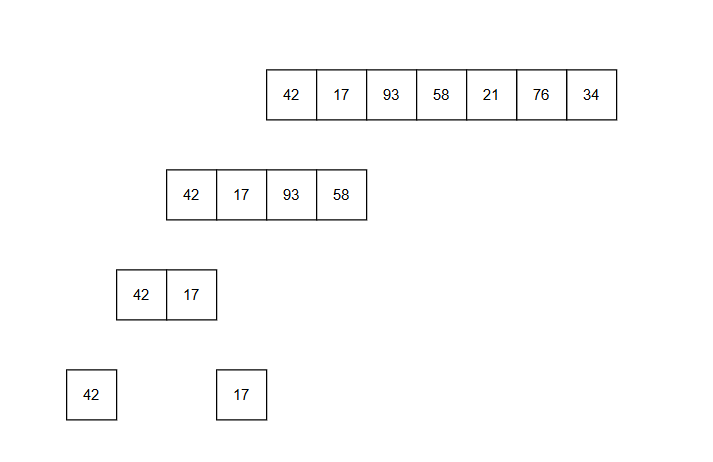
\includegraphics[width=0.7\textwidth]{img/merge_sort/1.png}
        \caption{Minh họa MergeSort-1}
    \end{figure}
    
    \item Trộn các phần tử đã chọn thành mảng sắp xếp:
    \begin{figure}[H]
        \centering
        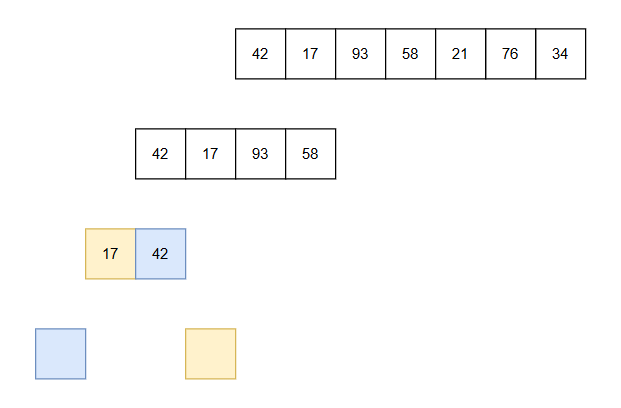
\includegraphics[width=0.7\textwidth]{img/merge_sort/2.png}
        \caption{Minh họa MergeSort-2}
    \end{figure}
    
    \item Gọi đệ quy cho nửa trái của nửa phải ban đầu:
    \begin{figure}[H]
        \centering
        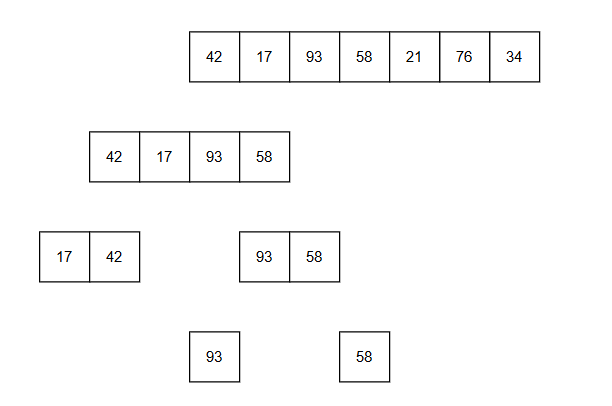
\includegraphics[width=0.7\textwidth]{img/merge_sort/3.png}
        \caption{Minh họa MergeSort-3}
    \end{figure}
    
    \item Trọn các phần tử đã chọn thành mảng sắp xếp:
    \begin{figure}[H]
        \centering
        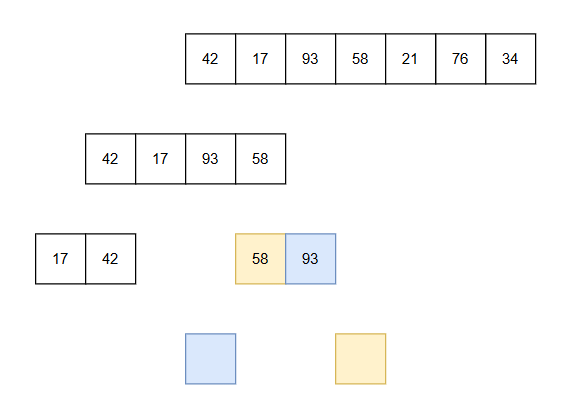
\includegraphics[width=0.7\textwidth]{img/merge_sort/4.png}
        \caption{Minh họa MergeSort-4}
    \end{figure}
    
    \item Trộn hai nửa của nửa phải mảng ban đầu thành mảng sắp xếp:
    \begin{figure}[H]
        \centering
        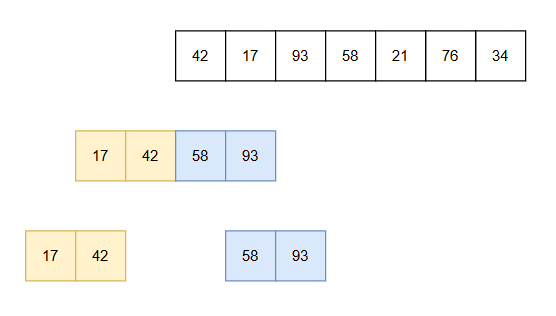
\includegraphics[width=0.7\textwidth]{img/merge_sort/5.png}
        \caption{Minh họa MergeSort-5}
    \end{figure}
    
    \item Gọi đệ quy tương tự cho nửa trái của mảng ban đầu:
    \begin{figure}[H]
        \centering
        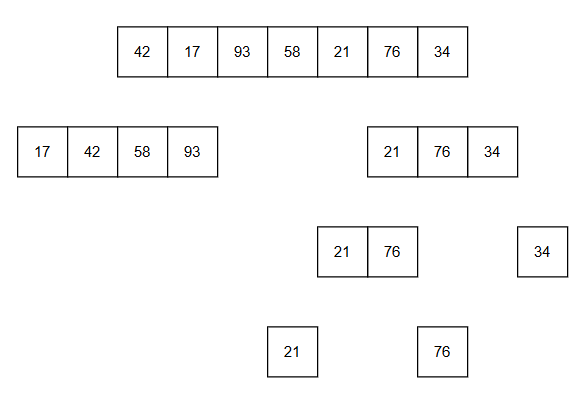
\includegraphics[width=0.7\textwidth]{img/merge_sort/6.png}
        \caption{Minh họa MergeSort-6}
    \end{figure}
    
    \item Trộn các phần tử đã chọn thành mảng sắp xếp:
    \begin{figure}[H]
        \centering
        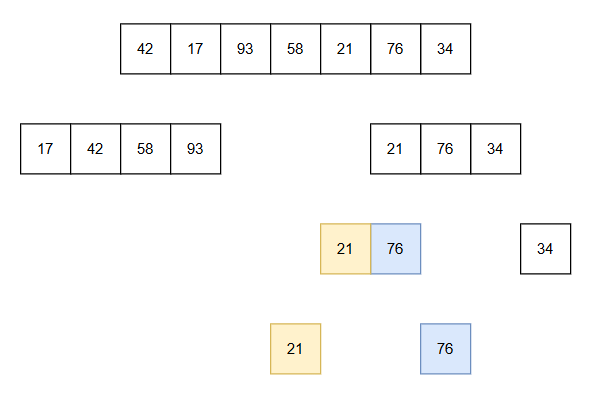
\includegraphics[width=0.7\textwidth]{img/merge_sort/7.png}
        \caption{Minh họa MergeSort-7}
    \end{figure}
    
    \item Trộn hai nửa của nửa trái mảng ban đầu thành mảng sắp xếp:
    \begin{figure}[H]
        \centering
        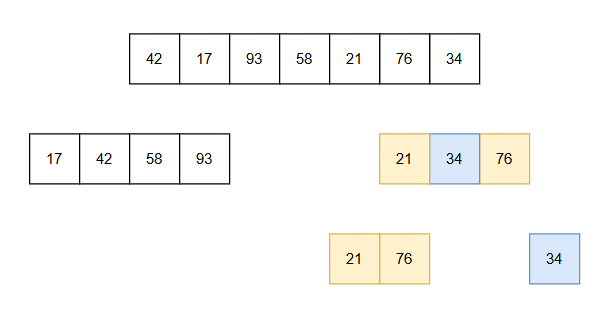
\includegraphics[width=0.7\textwidth]{img/merge_sort/8.png}
        \caption{Minh họa MergeSort-8}
    \end{figure}
    
    \item Trộn hai nửa của mảng ban đầu thành mảng sắp xếp:
    \begin{figure}[H]
        \centering
        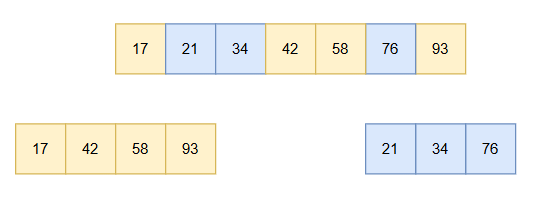
\includegraphics[width=0.7\textwidth]{img/merge_sort/9.png}
        \caption{Minh họa MergeSort-9}
    \end{figure}
    
    \item Hoành thành sắp xếp:
    \begin{figure}[H]
        \centering
        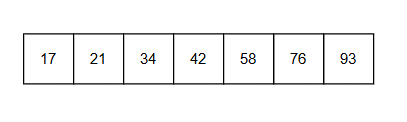
\includegraphics[width=0.7\textwidth]{img/merge_sort/10.png}
        \caption{Minh họa MergeSort-10}
    \end{figure}
\end{enumerate}

\subsubsection{Độ phức tạp}
\begin{itemize}
    \item[\textbf{--}] \textbf{Thời gian:}
    \begin{itemize}
        \item[$\bullet$] \textbf{Best Case:} \(\mathcal{O}(n \log n)\)
        \item[$\bullet$] \textbf{Average Case:} \(\mathcal{O}(n \log n)\)
        \item[$\bullet$] \textbf{Worst Case:} \(\mathcal{O}(n \log n)\)
    \end{itemize}
    \item[\textbf{--}] \textbf{Không gian:}
    \begin{itemize}
        \item[$\bullet$] Merge Sort yêu cầu bộ nhớ phụ trợ để lưu trữ các mảng con trong quá trình hợp nhất, do đó độ phức tạp không gian là:
        \[
        \mathcal{O}(n)
        \]
        \item[$\bullet$] Tổng không gian bộ nhớ: \(\mathcal{O}(n)\).
    \end{itemize}
    \item[\textbf{--}] \textbf{Tính ổn định:}
    \begin{itemize}
        \item[$\bullet$] Merge Sort là một thuật toán \textbf{ổn định}. Điều này có nghĩa là khi hai phần tử có giá trị bằng nhau, thứ tự ban đầu của chúng trong mảng sẽ không thay đổi trong quá trình sắp xếp.
    \end{itemize}
\end{itemize}